\chapter{Political Party Control and Intergovernmental Grants: a Panel Data Analysis}

\section{Introduction}

Fiscal federalism has long been a focal point within the realm of public finance, particularly concerning the strategic dynamics between various tiers of government\parencite{gordon1983optimal,dahlby1996fiscal,agrawal2022local}.
The allocation of intergovernmental transfers within this domain emerges as a critical area of inquiry, given its potential to profoundly influence governmental fiscal behavior and potentially lead to distortions\parencite{dahlby1996fiscal,gordon1983optimal}. For instance, these grants may induce overspending by subnational governments or stimulate/retard state governments' tax collection behavior\parencite{inman2008flypaper,bailey1998flypaper,turnbull1998overspending}. This paper seeks to unravel a fundamental question within the realm of American fiscal intergovernmental transfer: does the distribution of federal grants reflect the influence of party preferences and alignment between federal and state governments, as well as party attributes at the state level? These concerns pivot around the potential for federal bias favoring states with matching political affiliations, a significant inquiry given grants' role as 20\% of federal annual revenue \parencite{rosenstiel2021congressional}.


Empirical investigation into the grants allocation of funds has delineated the complex negotiations and compromises that characterize grant distribution---a process described not merely as top-down decisions, but as federative conciliation \parencite{chubb1985political, 1976A, dixit1995redistributive}. Our focus narrows upon federal decision-making, assuming the compliance of subnational governments---a perspective less explored but critical in the intricate hierarchy of government interactions. The traditional investigation on the bargaining on federal level, often based on game theory, propose rational, identical players \parencite{baron1989bargaining, banks2006general, martin2018dividing}, but the diversity of stakeholders involved introduces an array of additional considerations\parencite{milligan2005regional, golden2008pork,tellier2006public, petry1999electoral}.
Factors such as partisan alignment and preferences for grant categories are part of this multifaceted equation\parencite{rosenstiel2021congressional}, each contributing to the complex reality of grant distribution.

This paper seeks to address gaps in the literature by empirically investigating the effects of party preference and alignment between federal and state governments, as well as state party affiliation, on intergovernmental transfer distribution. In addition, we want to distinguish whether the alignment effect, if it's significant, is due to the federal level's subjective favoritism towards states with similar party affiliations. By dissecting panel data spanning various states and political contexts, this paper will highlight how such political dynamics manifest in the actual allocation of federal funds.

In Chapter 3, the dissertation takes a critical turn to explore the nuanced effects of political party control on the distribution and utilization of intergovernmental grants within the United States, a pivotal component of the fiscal federalism framework. This analysis directly supports the overarching aim of the dissertation to unravel the complex dynamics of fiscal interactions between central and subnational governments, by focusing on the political dimensions that underpin these interactions. By employing a panel data analysis over a 19-year period, this chapter sheds light on how political alignment and party control significantly influence the flow of intergovernmental transfers, adding a critical layer of understanding to the strategic fiscal behaviors of governments within the federal system. This exploration not only enhances our comprehension of fiscal federalism's theoretical and practical applications but also underscores the importance of political considerations in the design and execution of fiscal policies. As such, the findings from this chapter contribute to a more nuanced understanding of fiscal federalism and intergovernmental transfer, enriching the dissertation's holistic examination of governmental fiscal strategies and their implications for public service delivery across different tiers of government.

Following this introduction, a comprehensive overview of the grant distribution rules in the United States will set the platform for our narrative. We will then proceed with a robust literature review to carve out the missing pieces in the existing body of research. Our research questions and hypotheses will be postulated with precision and academic rigor, subsequently leading to a dialogue on our research methodology and an analysis of the findings in pursuit of academic and practical enlightenment.


\section{Background}

This section endeavors to demystify the landscape of intergovernmental grants within the intricate tapestry of the U.S. federal fiscal system. A clear comprehension of these transfers is vital for a holistic understanding of the factors, especially political, which may sway the distribution of grants across states.

Intergovernmental grants are instrumental in strengthening subnational entities, addressing the inequities propagated by fiscal decentralization—both vertical disparities rooted in structural differences and horizontal ones emanating from diverse fiscal capacities and expenditure requirements of jurisdictions. This multifunctional fiscal instrument is designed not only to instill spending in national-priority sectors but also to harmonize fiscal imbalances across regions.

In academic discourse, "transfers" and "grants" are terms historically employed with nuanced differences; with "transfers" being a broader term for resource shifts impacting revenue, while "grants" specify monetary allocations  \parencite{ter1997fiscal, Ahmad:1995,boadway1986federal}. Contemporary scholarship often unifies these terms, recognizing both as monetary exchanges between governmental tiers \parencite{abbott2012intergovernmental,lago2024effects,akai2019role}. In alignment with recent trends, this paper will use 'transfers' and 'grants' interchangeably to depict fiscal handovers from the federal to subnational levels.

In the U.S. financial regimen, grants are assorted primarily by two determinants as outlined in scholarly reviews\parencite{clemens2023intergovernmental, dilger2015federal}: the level of discretion bestowed upon federal administrators and the methodologies employed in quantifying grant shares. I will explore these dimensions to classify the grant types meticulously.

\subsection{1st Dimension: Degree of Federal Administrator}

Firstly, grants diverge in terms of federal discretion. From high level discretion to low, grants encompass categorical grants, block grants, and general revenue sharing grants.

\begin{itemize}
    \item{Categorical grants}
\end{itemize}

Categorical grants are money given to state and local governments for programs and projects with specific limitations on how that money is to be spent.
Categorical grants allocated funds may be spent only for narrowly defined purposes, thus federal government has highest discretion.

\begin{itemize}
    \item{Block grants}
\end{itemize}

signifying a relatively flexible pool of funds permitting regional authorities to tailor programs to local needs and provide flexibility to each subsidiary government body in terms of designing and implementing programs\parencite{finegold2004block}.

\begin{itemize}
    \item{General revenue sharing grants}
\end{itemize}

General revenue sharing, a government unit's apportioning of part of its tax income to other units of government. General revenue sharing grants, with minimal limitations, empower recipient governments to allocate funds as deemed fit. Laws determine the formulas by which revenue is shared; the units that receive the money are free from most controls by the granting unit, and the receiving units may or may not be required to match the amounts received\parencite{larkey2015evaluating}.

\subsection{2nd Dimension: Method of determining grant amounts}

Secondly, grants can differ based on the method of determining grant amounts, comprising project grants, formula grants, and reimbursement grants.

\begin{itemize}
    \item{Project grants}
\end{itemize}

Project grants involve competitive processes for grant allocation, encouraging states to propose and execute exemplary projects.


\begin{itemize}
    \item{Formula grants}
\end{itemize}

Formula grants are allocated to states based on mathematical formulas that take into account social characteristics within the jurisdiction\parencite{huffman2006formula}.

\begin{itemize}
    \item{Reimbursement grants}
\end{itemize}

Reimbursement grants reimburse state and local governments for a portion of their expenditures on specific programs, with open-ended and closed-ended matching grant variations.

These frameworks yield a spectrum of hybrid grant types and underscore the imperative of grasping their operational subtleties. Understanding these grant classifications lays the foundation for dissecting the intricate dynamics of grant distribution and their ramifications within fiscal federalism. In the following segments, we will delve into the traits of each grant class, examining their effects through empirical lenses. I present a two-dimensional matrix categorizing the grants, as illustrated in Figure \ref{grantstype}. According to the Congressional Research Service, around 600 grant programs exist, with categorical grants forming about 70\% of the total outlays\parencite{dilger2015federal}.

% \begin{figure}[H]
%     \centering
%     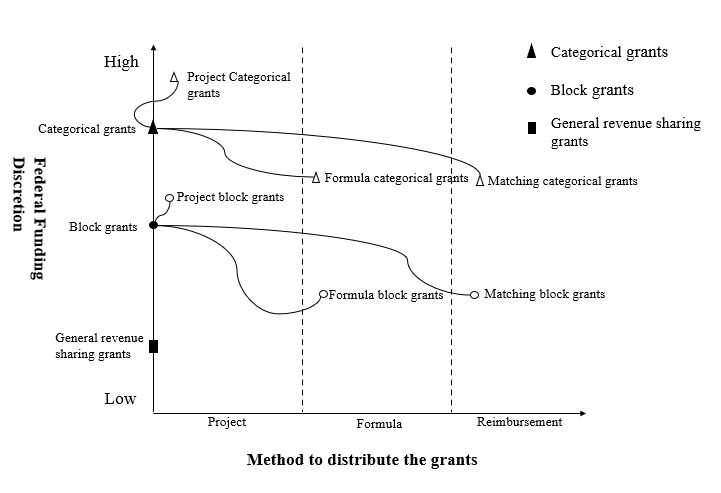
\includegraphics[scale=0.8]{Chapter-3/Figures/grants type.JPG}
%     \caption[Grants Type in America]{Grants Type in America
%         \texttt{} }
%     \label{grantstype}
% \end{figure}

Our nuanced classification elucidates the potential channels through which federal decision-making might deliberately skew grant allocations. With project grants, federal influence is at its zenith, having the authority to select recipients and set amounts directly. Formula grants afford a subtler federal influence, where selection criteria embedded in the formulas can be oriented to favor certain constituencies. Reimbursement grants, while not as directly controlled, allow the federal government to dictate the subsidizable realms and the extents, thereby steering benefits towards preferred states.

%%%%%%%%%%%%%%%%%%%%%chatgptchecked%%%%%%%%%%%%%%%%%%%%%%%%%%%%%%%%%%%%%%%%%%%%

\section{Literature Review}

The purpose of this section is to introduce and analyze existing literature relevant to the research problem addressed in this study, aiming to elucidate the theoretical frameworks and empirical findings that inform our understanding of intergovernmental transfer decision-making processes in the United States. In particular, this review aims to place our research within the broader academic conversation on intergovernmental grants. It will emphasize key theoretical insights and empirical observations directly relevant to our investigation of factors influencing grant distribution outcomes in the American context.

Moreover, through a summary of the literature, we identify a potential correlation between the allocation of transfer payments and the combined party affiliations at both central and local levels. This correlation raises the question: is it driven by federal-level favoritism towards states sharing the same party affiliation, or is it a consequence of federal decision-makers aiming to assist specific states (e.g., the one they represent), leading states with similar political and social characteristics to also benefit as "free riders" due to their shared party affiliation? This presents a central challenge in discerning the impact of the "joint distribution of federal and state party affiliations" on the distribution of transfer payments.

In the realm of intergovernmental transfer decision-making, existing literature, as reviewed, can be broadly categorized into two streams: theoretical investigations and empirical analyses. The former encompasses formal theoretical game theory analyses, delving into abstract bargaining processes and proposing conjectures based on various assumptions. Over time, theoretical research has evolved, with hypotheses increasingly aligning with administrative reality, yielding more practically meaningful conclusions. The latter category aims to explore potential factors influencing the outcomes of intergovernmental transfers, primarily through empirical investigations, typically found in public administration, political science, and certain areas of applied economics.

\subsection{Review on Theoretical Investigation}

The distribution of grants in democratic countries is considered a bargaining game among decision-making groups, such as committees, congress, depending on which group is the decisive institution. \textcite{baron1989bargaining}'s model of the legislature is considered foundational and seminal in this field and following investigation somewhat follows \textcite{baron1989bargaining}'s framework. In Baron and Ferejohn's framework, four assumptions are crucial in simulating the grants distribution bargaining: the recognition rule, voting rule, amendment rule, and money-distribution rule.

The recognition rule determines how to select an agenda setter to make the initial proposal, with most literature assuming the random recognition rule. This means that $n$ members among the decision-making institution have equal probabilities of being chosen to make the initial proposal \parencite{kalandrakis2004three,anesi2015bargaining,diermeier2011legislative,rosenstiel2021congressional}.

The voting rule establishes the standard for passing the proposal, with the majority rule and unanimous voting rule being common. The amendment rule places constraints on making amendments, ranging from the closed rule (allowing no amendments) to the open rule (allowing any and all germaine amendments).

Finally, the grants-type rule determines how grants could be manipulated by decision-making institutions, with some scholars assuming direct decisions on the number of receivers, referred to as "earmarks" spending models. %%chatgpt checked%%%

\Textcite{baron1989bargaining} laid the foundation for subsequent analyses of bargaining models. They made several important assumptions, such as random recognition, majority voting rule, and earmarks rule. Their work, as well as the generalization by \Textcite{banks2006general}, demonstrates that legislators with agenda-setting power tend to receive a disproportionate share of funding. In addition, the equilibrium is characterized by funds flowing only to legislators in the winning coalition, with no funds allocated to those outside of it. Furthermore, they found that when proposals are brought up under a closed rule, the winning coalition is minimized, leading to the maximization of benefits for the members of the winning coalition.

\Textcite{baron1989bargaining}'s work is pioneering in the field of grants distribution, but its heavy reliance on the "earmarks" assumption limits its explanatory power in the actual political environment. \Textcite{martin2018dividing} addresses this issue by modifying the assumptions of the model. Specifically, he restricts the power of decision-making members to only determine the factors in the formula rather than the specific numbers. This modification is a significant step towards reflecting the realities of political and administrative life.

\textcite{martin2018dividing}'s model generates different conclusions compared to Baron and Ferejohn's work. In contrast to the latter, Martin predicts oversized winning coalitions and the emergence of persistent winning blocs. Additionally, he demonstrates that when bargaining over a low-dimensional formula, legislators have limited ability to target funds to specific districts, a prediction supported by empirical evidence. For instance, Martin analyzed existing formula grants and found that 95\% of the formulas have fewer than 5 variables, indicating limited bargaining dimensions for members. Consequently, some jurisdictions can be free-riders, even if they are not part of the winning coalition. Martin predicts positive distribution outside the winning coalition as a consequence.

In conclusion, theoretical analyses in game theory have evolved towards reflecting the realities of government governance. While theoretical research has made significant contributions to understanding government behavior, it may overlook the role of variables that deviate from basic assumptions, such as party affiliation, party preference, or alignment between federal and state levels.

Moreover, if we do find the correlation between grants distribution and alignment between federal and state governments, attributing the influence of party factors solely to subjective motives at the federal government level may be overly simplistic. For instance, legislators from Republican states advocating for Republican interests could be driven by a subjective preference for the party or a desire to advocate for their state's interests, with states with similar characteristics choosing to be free riders. As Martin suggests the potential existence of a free rider effect, grants may flow to recipients other than the winners regardless of subjective motives.

\subsection{Review on Empirical Investigation}


Beyond the introductory considerations of intergovernmental transfers in theoretical investigations, a primary challenge in their distribution lies in the political environment where such allocations transpire.  For instance, in the context of the United States, it is crucial to examine the divergent impacts when different political parties prevail in negotiations and discern the role of partisanship within subnational governments.In conclusion, the intricate interplay of politics significantly influences the allocation of intergovernmental transfers, warranting a comprehensive understanding of the distribution mechanisms, particularly in the American context.

Given the pivotal role of intergovernmental transfers in the U.S. federal system, the impact of politics on their allocation can be excessively influencing. Various anecdotal examples underscore this phenomenon, including the protracted efforts of Robert Carlyle Byrd to channel federal spending to his home state, West Virginia, spanning two decades. One notable instance of Byrd's influence manifests in the formulation of a new distribution formula for a trust fund surplus, proposed by him during the 1992-1997 authorization negotiations. This recalibrated formula predominantly favored states with elevated state gasoline tax rates and diminished per capita income, with West Virginia standing as a pertinent beneficiary.%%%%chatgpt checked%%%

\textcite{markusen1981benefits} conducted a descriptive study analyzing three distinct shifts in the distribution of federal grants to cities during the 1960s and 1970s. The research revealed a substantial increase in federal grants during this period, with northeastern and midwestern cities benefiting the most from 1965-1972, southern and western cities from 1972-1975, and a slight return in favor of the first group from 1975-1978. These variations can be partially attributed to the political landscape. \textcite{stegarescu2006decentralised} explains that the degree of Intergovernmental Transfer (IGT) decentralization is influenced by population, unemployment, trade openness, presidential regimes, and electoral systems. This conclusion is drawn from panel data analysis encompassing 17 nations. Empirical testing by \textcite{kasdin2016decision} revealed that the complexity of state or local government networks affects the amount of federal transfers and federal control. Higher-level governments tend to relinquish control in the presence of a complex lower governmental network. However, the amount of transfer is negatively correlated with complexity. Complexity acts as a barrier hindering politicians from claiming political credit, reducing their motivation to secure fiscal revenue for their jurisdiction. \textcite{larcinese2006allocating} examined the impact of presidential support on federal transfers to state governments. Their findings indicate that states strongly supporting the incumbent president in past elections tend to receive more funds. \textcite{wallis1987employment} underscores that states with high volatility in presidential voting receive significantly more federal support. This conclusion is drawn from a longitudinal study encompassing all states in the U.S. \textcite{markusen1981benefits} proposed a comprehensive framework defining the supply and demand sides when investigating the mechanism of Intergovernmental Transfers (IGTs) decision-making processes. They highlight that IGTs result from the political, economic, and social characteristics of both the demand and supply sides.


To summarize, our literature review provides evidence for the necessity of our study on intergovernmental transfer decision-making processes in the United States. While theoretical research offers valuable insights into grant distribution dynamics, it inherently simplifies and abstracts complex realities, potentially overlooking crucial factors such as the preferences of different parties, branches of government, and alignment between different levels of government. Conversely, empirical analyses highlight the significant impact of various factors on grant distribution outcomes in real administrative processes.

Nevertheless, our review also highlights the challenges associated with exploring the influence of factors like party preferences and alignment between levels of government. While confirming the existence of these influences may be relatively straightforward, discerning whether they stem from subjective preferences and cooperation among party allies or unintended outcomes due to shared economic and social characteristics among same-party states poses greater difficulty. Therefore, our subsequent research endeavors to address these challenges by examining the economic and social attributes of same-party states and evaluating the extent to which political factors are influenced by objective economic and social characteristics. Through meticulous control of these factors, we aim to offer a nuanced understanding of the complexities underlying intergovernmental transfer decision-making in the United States.


\section{Problems and Hypothesis}

This section serves as a statement of problems and our hypotheses, outlining the issues addressed and conjectures made in our study. Building upon our prior analysis and literature review, as well as recognizing potential challenges, our inquiries are structured in two steps. Firstly, we aim to investigate whether there are commonalities or differentiations in the socioeconomic characteristics of same-party and different-party states. This inquiry helps elucidate whether the apparent preferences of the federal decision-making level towards specific party-state groups may result from non-subjective motives, as these "preferences" may not necessarily stem from subjective intentions\parencite{martin2018dividing}. Following the resolution of this question, we can delve into exploring the effects of factors such as party affiliation, party preference, and alignment on grant distribution. Specifically, our study seeks to address five key questions.


\subsection{Problems}
The questions of interest are as follows:

\begin{itemize}
    \item  Does states from same partisanship share similar social and economic features, which tend to be part of the grants distribution formula?
\end{itemize}

One potential conjecture is: subnational jurisdictions with same partisanship may share similar social and economy features.

\begin{itemize}
    \item  The distribution of Intergovernmental Transfers (IGT) is influenced by the unity of legislative and administrative branches at the central level.
\end{itemize}


The term "unity" here refers to the situation where both the administrative and legislative branches are controlled by the same party. A body of empirical evidence indicates that the executive and legislative branches typically harbor distinct policy intentions. This divergence implies potential hindrances to intergovernmental transfer programs when these branches are separately controlled by different political parties \parencite{peterson1994executive,carreras2014outsiders, farhang2012legislative}. Such discrepancies should manifest in the overall amounts of intergovernmental transfers.

\begin{itemize}
    \item Whether the Democratic and Republican parties exhibit divergent preferences in the distribution of Intergovernmental Transfers (IGT).
\end{itemize}

The impact of partisanship on intergovernmental transfers can be examined from two perspectives: the party's inclination towards spending tendencies and the party's stance on decentralization \parencite{dinan2020stability, freeman1986political}.

\begin{itemize}
    \item Whether a swing states receives more IGT.
\end{itemize}

The central government at the national level may potentially be inclined to provide additional grants to swing states in order to secure crucial support in electoral competitions.

\begin{itemize}
    \item Whether the alignment of party between the federal and state governments affects the grants amounts.
\end{itemize}

The central government may exhibit a preference for allocating resources to states controlled by the same party as the central government.

Following the problems we made, we construct our hypothesis.

\subsection{Hypothesis}

There are five hypothesis in this investigation. Each hypothesis corresponds to one of the previously mentioned questions.

\textbf{Hypothesis 1: The Same-Party State Consistency Hypothesis}

This hypothesis posits that states governed by the same political party exhibit similar economic and social attributes. Numerous American and international studies have provided evidence indicating that factors such as economic structure and economic conditions influence political affiliation. Therefore, it is plausible to infer that the reverse logic holds true: regions governed by the same political party may also share similar economic and social structures \parencite{Alan2009Partisanship,2006Economic, 62b81da7-cc78-33f9-98a3-0a8d03976c2c}.

\textbf{Hypothesis 2: The unified Government Hypothesis}

A unified government is characterized by the alignment of the administrative branch and legislative branch at the federal level under the same political party. This alignment tends to result in higher overall spending, as the convergence of executive and legislative powers reduces financial constraints.

\textbf{Hypothesis 3: Party Specific Hypothesis}

The Democratic and Republican parties exhibit distinct preferences regarding the scale of Intergovernmental Transfers (IGT). Interpreting party preferences in this context is nuanced, as two plausible inferences can be drawn. Regarding the size of government, the Democratic Party tends to favor a larger government, resulting in higher-scale IGT. Conversely, the Republican Party holds the opposing view. In terms of administrative structure, Democratic governments tend to favor a centralized system, while Republican governments prefer a decentralized structure. Consequently, these contrasting perspectives lead to divergent conclusions.

\textbf{Hypothesis 4: Alignment Hypothesis}

The distribution of intergovernmental transfers (IGT) is influenced by political affiliation. There is a tendency for the federal government to allocate more IGT to states controlled by the same political party.

\textbf{Hypothesis 5: Battle Ground States Hypothesis}

The federal government, driven by the motivation to secure election or reelection, is inclined to allocate resources and provide additional public goods to states that significantly influence electoral outcomes. This strategic allocation is aimed at accruing political credits. Therefore swing states are easier to get more grants.

\section{Research Method Design}


To validate the aforementioned hypotheses and address related questions, I employed two research methods to address different issues. The selection of these two methods was based on the distinct research requirements of each question. For the first question, I needed to analyze the economic and social characteristics associated with different political party affiliations, in another word, I need to analyze similarity among states governed by the same party regarding social and economic factors. For questions 2 through 5, I needed to conduct regression analysis while controlling for economic and social variables. The relationship between the political factors and IGT amounts is solved through a panel data regression.

Therefore, the research methods are listed as two parts. The first part talks about the method to analyze the relationship between social, economic factors and partisanship; another method is a regression model to investigate the effect of the preference of different parties, different branches or the alignment between different levels of governments.

\subsection{Method on the First Question--Principal Components Analysis (PCA)}
\subsubsection{Data and variables for PCA Analysis}
In the first research method employed in this study, the primary variables required mainly consist of economic and social characteristics at the state level, with particular emphasis on variables frequently appearing in transfer payment formulas. Additionally, as this article specifically focuses on the economic and social commonalities among states governed by the same political party, a grouped sampling method was adopted for selecting sample states. All states were categorized into traditional Democratic states, traditional Republican states, and traditional swing states. Within each group, 5-6 states were randomly selected as samples. The economic and social variables of all selected sample states were then analyzed for annual changes from 2000 to 2019, thus forming a panel dataset.

The state grouping method relies on two primary criteria: historical presidential election outcomes and their corresponding winning percentages, a methodology delineated in \textcite{beachler2015presidential}. Democratic and Republican states are characterized as those consistently favoring a particular party in presidential elections since 1984, where the winning rates surpass 58\%. Swing states are recognized as those that have alternated between parties in selecting presidents, with winning rates falling below 58\%. The states encompassed within the analysis are enumerated in Table \ref{Table 2.3}.

% Table generated by Excel2LaTeX from sheet1.
% \begin{table}
%     \caption{States Sample and Grouping}
%     \begin{tabular}{p{7.57em}cc}
%         \toprule
%         States         & \multicolumn{1}{p{7.93em}}{Group}                    & \multicolumn{1}{p{6.855em}}{Code} \\
%         \midrule
%         Wyoming        & \multicolumn{1}{c}{\multirow{5}[2]{*}{Red States}}   & \multirow{5}[2]{*}{1}             \\
%         Idaho          &                                                      &                                   \\
%         Kansas         &                                                      &                                   \\
%         Nebraska       &                                                      &                                   \\
%         North Dakota   &                                                      &                                   \\
%         \midrule
%         Maryland       & \multicolumn{1}{c}{\multirow{5}[2]{*}{Blue States}}  & \multirow{5}[2]{*}{2}             \\
%         Massachusetts  &                                                      &                                   \\
%         Rhode Island   &                                                      &                                   \\
%         New York State &                                                      &                                   \\
%         Washington     &                                                      &                                   \\
%         \midrule
%         Pennsylvania   & \multicolumn{1}{c}{\multirow{4}[2]{*}{Swing States}} & \multirow{4}[2]{*}{3}             \\
%         Nevada         &                                                      &                                   \\
%         Wisconsin      &                                                      &                                   \\
%         Ohio           &                                                      &                                   \\
%         \bottomrule
%     \end{tabular}%
%     \label{Table 2.3}%
% \end{table}%


The social and economic characteristics commonly included in the formula for intergovernmental transfers encompass population, working-age population weight, median household income, unemployment rate, road mileage, and GDP per capita \parencite{dilger2015federal}. I gathered all factors mentioned in \Textcite{dilger2015federal}'s study for the sampled states. Additionally, I referenced major intergovernmental transfer programs such as Medicaid, the Title I-A education program, Temporary Assistance for Needy Families (TANF), Section 8 Housing Choice Vouchers, and the Community Development Block Grant (CDBG) to comprehensively collect factors. To ensure data convenience for regression and enhance data visualization, I performed appropriate operations. The collected characteristics and data sources are detailed in Table \ref{Table 2.4}.%%%%%%chatgpt checked%%%%%

% \begin{table}
%     \centering
%     \caption{Social characteristics for Sample States}
%     \begin{tabular}{cp{6.43em}p{9.285em}p{5.855em}p{5.355em}}
%         \toprule
%         \multicolumn{1}{p{4em}}{Variables } & Definition                      & Operation          & Source                              & Time Period                  \\
%         \midrule
%         gdp                                 & \multicolumn{1}{c}{Real GDP}    & Log transformation & FRED                                & 2000-2019 annually collected \\
%         \midrule
%         lgp                                 & \multicolumn{1}{c}{Population } & Log transformation & Census of bureau                    & 2000-2019 annually collected \\
%         \midrule
%         wapw                                & Working age population weight   & No operation       & Census of bureau                    & 2000-2019 annually collected \\
%         \midrule
%         mhi                                 & State median household income   & Log transformation & Census of bureau                    & 2000-2019 annually collected \\
%         \midrule
%         ur                                  & unemployment rate               & No operation       & FRED                                & 2000-2019 annually collected \\
%         \midrule
%         prm                                 & public road mileage             & Log transformation & Bureau of transportation statistics & 2000-2019 annually collected \\
%         \bottomrule
%     \end{tabular}%
%     \label{Table 2.4}%
% \end{table}%

\subsubsection{PCA Process}
As previously mentioned, the formula for distributing grants may encompass numerous factors. Additionally, issues of correlation are evident within the collected variables. For example, the weight of the working-age population and the unemployment rate are highly interdependent variables and higher population levels inherently correspond to increased usage of public roads. This observation is further corroborated by the correlation heatmap in figure \ref{heatmap}, which indicates a certain degree of correlation among the variables. To compare the similarities of social and economic conditions among same partisanship states, correlation issue need to be fixed and data dimension reduction is necessary.%%%%%chatgpt checked%%%%%

% \begin{figure}
%     \centering
%     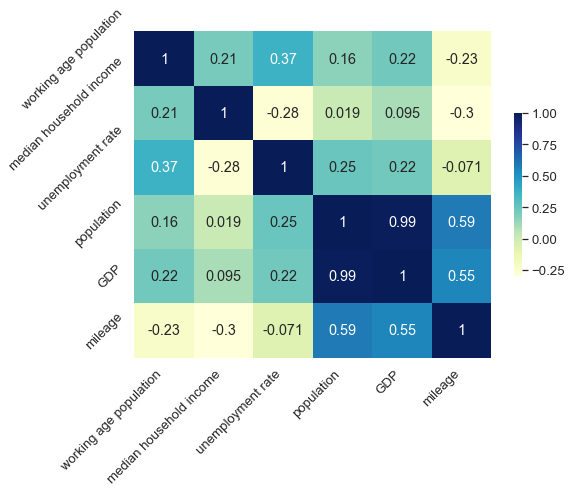
\includegraphics[scale=0.7]{Chapter-3/Figures/heatmap.png}
%     \caption[Heatmap of the Social Characteristics]{Heatmap of the Social Characteristics
%         \texttt{} }
%     \label{heatmap}
% \end{figure}

To address the first question, the apparent hindrance lies in the difficulty of directly assessing the similarity of jurisdictions in social and economic characteristics. To overcome this challenge, I employed Principal Components Analysis (PCA) to reduce data dimensionality and mitigate issues of multicollinearity. This approach aims to determine whether the reduced-dimension data exhibit cluster distribution or scattered distribution.

The results of the PCA variance analysis, as depicted in the figure, reveal that the first two dimensions encapsulate 67\% of the information, while the first three dimensions account for 87\% of the information.
% \begin{figure}[H]
%     \centering  %居中
%     \subfigure[Histgram]{   %第一张子图
%         \begin{minipage}{7cm}
%             \centering    %子图居中
%             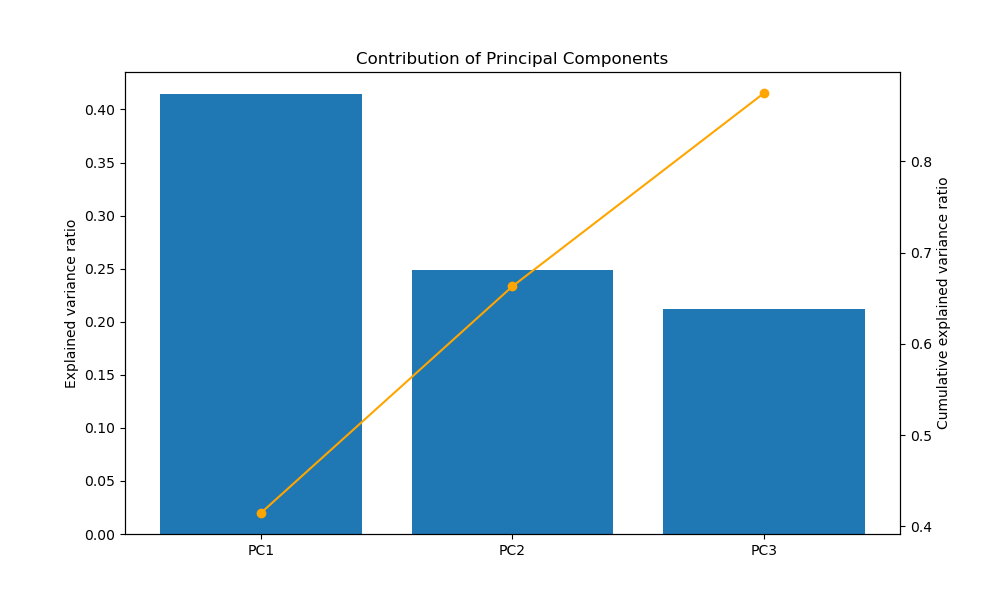
\includegraphics[scale=0.2]{Chapter-3/Figures/contribution.png}  %以pic.jpg的0.5倍大小输出
%         \end{minipage}
%     }
%     \subfigure[Line]{ %第二张子图
%         \begin{minipage}{7cm}
%             \centering    %子图居中
%             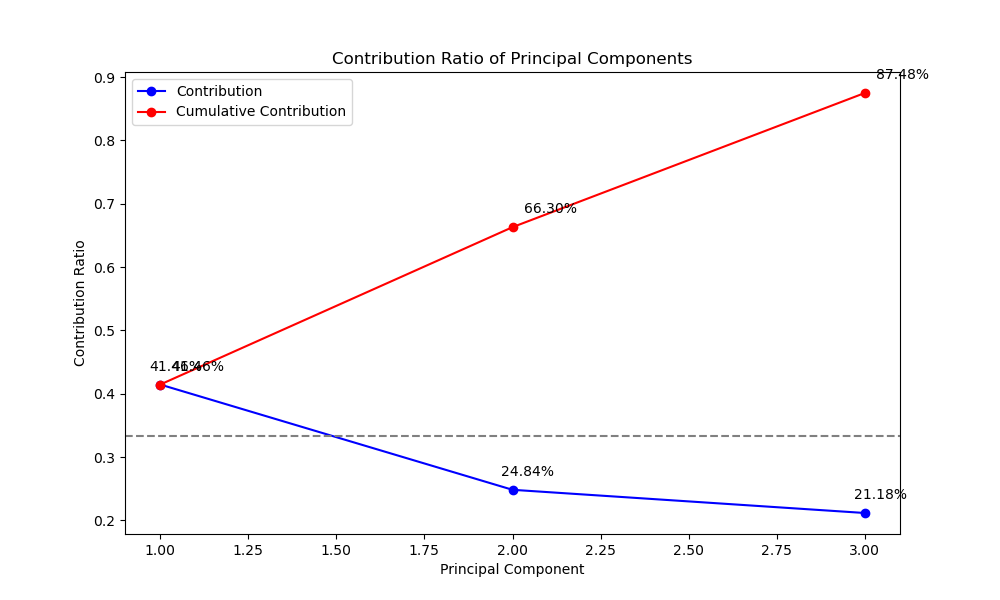
\includegraphics[scale=0.2]{Chapter-3/Figures/contribution2.png}%以pic.jpg的0.5倍大小输出
%         \end{minipage}
%     }
%     \caption[Principle Components Contribution]{Principle Components Contribution}    %大图名称
%     \label{principlecomponentcontribution}    %图片引用标记
% \end{figure}

Consequently, Principal Components Analysis (PCA) was employed to reduce the data into two and three dimensions separately. By retaining the two and three principal components with the highest information content, it became feasible to compare the characteristics between jurisdictions.

\subsection{Method on Question 2 to 5--Fixed Effect Regression}
\subsubsection{Data and variables}
Stratified sampling is also adopted, thus the sample states selected in the regression are same as the ones in PCA analysis and are grouped into traditional Republican states, traditional Democratic states, and swing states.

In terms of the variables, the dependent variable is the annual total intergovernmental transfer amount received by state $i$ in the United States. The total amount underwent a logarithmic transformation. The independent variables include $c$---alignment combination and $p$, which represent partisanship. Notably, the dummy variable $c$ represents the party distribution combination in the administrative and legislative branches across federal and state levels. Three key factors determine the nature of "$c$": the governmental level, branches, and different parties. A $2\times2$ table (Table \ref{Table 2.6}) is formed with two branches and two levels, resulting in four sectors denoted as $u_1, u_2, s_1, s_2$. Each sector has two possible parties in control, namely the Democratic party "$d$" and the Republican party "$r$".

For instance, $c_1 = (u_1 = r, u_2 = r, s_1 = r, s_2 = r)$ represents combination one, and is abbreviated as $(r, r, r, r)$. In this study, the majority in the House of Representatives defines the partisan composition of the legislative branch, given its pivotal role in the budget-making process. The partisan composition of the administrative branch is determined by the partisan affiliation of the administrative leader, who could be the president or governor. There are 16 types of combinations in $c$:

$$(r, r, r, r), (r, r, r, d), (r, r, d, r), (r, r, d, d), (r, d, r, r), (r, d, r, d), (r, d, d, r), (r, d, d, d)$$\\$$(d, r, r, r), (d, r, r, d), (d, r, d, r), (d, r, d, d), (d, d, r, r), (d, d, r, d), (d, d, d, r), (d, d, d, d) $$

I employ $c_1, c_2, . . . c_{16}$ to denote the 16 distinct combinations. In the regression analysis, only fifteen combinations are retained, with the omission of the first combination $c_1 = (r, r, r, r)$ to mitigate multicollinearity issues. $c_1$ serves as the benchmark in the regression model.

% \begin{table}[H]
%     \centering
%     \caption{Branches and Levels Combination}
%     \begin{tabular}{cp{7.145em}p{8.43em}p{6.145em}}
%         \toprule
%         \multicolumn{2}{c}{\multirow{2}[4]{*}{}}       & \multicolumn{2}{p{14.575em}}{Branches}                 \\
%         \cmidrule{3-4}    \multicolumn{2}{c}{}         & administrative                         & house         \\
%         \midrule
%         \multicolumn{1}{c}{\multirow{2}[4]{*}{Levels}} & federal                                & $u_1$ & $u_2$ \\
%         \cmidrule{2-4}                                 & state level                            & $s_1$ & $s_2$ \\
%         \bottomrule
%     \end{tabular}%
%     \label{Table 2.6}%
% \end{table}%


In the regression analysis, I incorporate a 1-time period lag of $c$ as an independent variable. The rationale behind this is that the general decision-making process is time-consuming, implying that the effect of a specific party combination $c$ should not be significant in the current year.

Regarding the dummy variable $p$, I gathered longitudinal data for three distinct types of states based on their political affiliations: traditional Democratic states, Republican states, and swing states. The 14 states are categorized into three groups. The first group constitutes the traditional Republican states, often referred to as the "red wall states," and we designate $p = 1$ for this group. The second group comprises traditional Democratic states, also known as the "blue wall states," and $p = 2$ is assigned to this group. The third group represents swing states, commonly referred to as the "battleground states," with $p = 3$ assigned to this category. The sampled states in this research align with those used in the principal components analysis, as outlined in Table \ref{Table 2.3}.


The control variables encompass prevalent social and economic factors integrated into the distribution formula for federal grants projects. These factors, identified in the literature, can be inferred to have an impact on grants distribution.


The collected variables are outlined in Table \ref{Table 2.5}, covering the period from 2000 to 2019. For further details, including data sources and specific information, please consult Appendix Table \ref {Table A.1}.

% \begin{table}
%     \centering
%     \caption{Variables and Operation}
%     \begin{tabular}{lcp{12.715em}p{6.145em}}
%         \toprule
%         \multicolumn{2}{p{9.93em}}{Variables }                        & Definition & Operation                                                                                    \\
%         \midrule
%         \multicolumn{1}{p{4.715em}}{Dependent Variable}               & lg(igt)    & IGT from federal to state i                               & Log                              \\
%         \midrule
%         \multicolumn{1}{l}{\multirow{2}[4]{*}{Independent Variables}} & c          & Combinations of levels, branches and parties.             & \multirow{2}[4]{*}{No operation} \\
%         \cmidrule{2-3}                                                & p          & Dummies to identify i is democratic, republican or swing. & \multicolumn{1}{c}{}             \\
%         \midrule
%         \multicolumn{1}{l}{\multirow{6}[12]{*}{Control Variables}}    & log(gdp)   & \multicolumn{1}{l}{Real GDP}                              & \multirow{4}[8]{*}{Log }         \\
%         \cmidrule{2-3}                                                & log(pl)    & \multicolumn{1}{l}{Population }                           & \multicolumn{1}{c}{}             \\
%         \cmidrule{2-3}                                                & wapw       & Working age population weight                             & \multicolumn{1}{c}{}             \\
%         \cmidrule{2-3}                                                & mhi        & State median household income                             & \multicolumn{1}{c}{}             \\
%         \cmidrule{2-4}                                                & ur         & unemployment rate                                         & No operation                     \\
%         \cmidrule{2-4}                                                & prm        & public road mileage                                       & Log                              \\
%         \bottomrule
%     \end{tabular}%
%     \label{Table 2.5}%
% \end{table}%
\subsubsection{Fixed Effect Regression}
Despite conducting a relatively comprehensive literature review on the issue of grants distribution formulas and incorporating sample data that addresses key concerns in intergovernmental transfer distribution, the possibility remains that some variables may have been omitted from the equation, particularly given the longitudinal nature of the data spanning 19 years. Consequently, a crucial challenge in this investigation is addressing potential omitted variable issues and avoid subsequent heteroscedasticity problems.

With panel data spanning 19 years, I adopt fixed effect model to overcome potential omitted variables. Besides, to minimize potential heteroscedasticity issues in subsequent analysis, robust standard error is employed
%%%%%%%%%%%%%%%%%%%%%%%%%%%%%%%%%%%%%%%%%%%%%%%%%%%%%%

In the subsequent research, I present three regression models. The benchmark model is an Ordinary Least Squares (OLS) regression with robust standard error. Additionally, the second model is a time factor and individual factor fixed regression. The third model is a individual variable fixed model.
%%%%%%%%%chatgpt checkedddd%%%%%%%%%%%%%%%%%%%%%%%%%%%%%%%%%%%%%%%%%%%%%%%%%%%%%%%


The equation for OLS regression can be displayed as follow:

\begin{equation}
    \begin{split}
        log(igt_{i,t}) & = \alpha + \beta_1 c_{i,t-1} + \beta_2 p_{i,t} + \beta_3 log(gdp) + \beta_4 log(pl) + \beta_5 log(mhi_{i,t}) \\
        & + \beta_6 wapw_{i,t} + \beta_7 ur_{i,t} +\beta_8 log(prm_{i,t}) + \epsilon_{i,t}
    \end{split}
\end{equation}
$For\ t = 1, 2, 3...T\ and\ i = 1, 2, 3...N $

The second model, which is the fixed effect model with time and state fixed is:
\begin{equation}
    \begin{split}
        log(igt_{i,t}) & = \alpha_i + \theta_t + \beta_1 c_{i,t-1} + \beta_2 p_{i,t} + \beta_3 log(gdp) + \beta_4 log(pl) + \beta_5 log(mhi_{i,t}) \\
        &+ \beta_6 wapw_{i,t} + \beta_7 ur_{i,t} +\beta_8 log(prm_{i,t}) + \epsilon_{i,t}
    \end{split}
\end{equation}
$For\ t = 1, 2, 3...T\ and\ i = 1, 2, 3...N $

Finally, the third model, which is states fixed effect model with state partisanship controlled is:

\begin{equation}
    \begin{split}
        log(igt_{i,t}) & = \alpha_i + \beta_1 c_{i,t-1} + \beta_2 p_{i,t} + \beta_3 log(gdp) + \beta_4 log(pl) + \beta_5 log(mhi_{i,t}) \\
        &+ \beta_6 wapw_{i,t} + \beta_7 ur_{i,t} +\beta_8 log(prm_{i,t}) + \epsilon_{i,t}
    \end{split}
\end{equation}
$For\ i = 0,1,2...N$.

%%%%%%%%chatgpt checked%%%%%%%%%%%%


\section{Result analysis}

Principal Components Analysis (PCA) was employed to reduce the data into two and three dimensions separately.The resulting scatter plot following data dimension reduction is presented in Figure \ref{Figure 2.2}.

% \begin{figure}[H]
%     \centering  %居中
%     \subfigure[2 Principle Components Analysis Scatter]{   %第一张子图
%         \begin{minipage}{7cm}
%             \centering    %子图居中
%             \includegraphics[scale=0.45]{Chapter-3/Figures/pca.png}  %以pic.jpg的0.5倍大小输出
%         \end{minipage}
%     }
%     \subfigure[3 principle Components Analysis Scatter]{ %第二张子图
%         \begin{minipage}{7cm}
%             \centering    %子图居中
%             \includegraphics[scale=0.45]{Chapter-3/Figures/pca_3d.png}%以pic.jpg的0.5倍大小输出
%         \end{minipage}
%     }
%     \caption[Principle Components Analysis Scatter Plot]{Social Characteristics Principle Components Analysis Scatter Plot}    %大图名称
%     \label{Figure 2.2}    %图片引用标记
% \end{figure}
%%chatgpt checked%%%%%

Although the reduced dimensions lack specific economic meaning, a notable observation in Figure \ref{Figure 2.2} is that many state characteristics exhibit a cluster distribution. In both two-dimensional and three-dimensional plots, the red, blue, and green points exhibit distinct distributions, with each color forming its own cluster. This suggests that states governed by the same political party share similar economic and social characteristics, which are notably different from those of states governed by other parties. In summary, principal component analysis results indicate a high level of cohesion within states governed by the same party in terms of their economic and social characteristics, while significant differentiation exists between states governed by different parties.

Such findings align with \Textcite{martin2018dividing}'s proposition that jurisdictions with similar features with winner players in the bargaining game may act as free riders, consequently predicting the outflow of funds from the winning coalition.

Another potential implication arises from the hierarchical distribution based on political parties. Republican states, Democratic states, and swing states exhibit distinct cluster distributions in their respective areas. In the 2D plot presented in Figure \ref{Figure 2.2} (a), red and blue dots are situated on opposing sides, with swing states occupying the intermediary position. This configuration implies that any modification to the grants formula favoring one party inflicts significant harm on another. This observation may elucidate the sharp opposition between the two parties during legislative bargaining, while swing states remain relatively indifferent. The distinctive nature of swing states is further illuminated in the 3D plot depicted in Figure \ref{Figure 2.2} (b), where green dots do not align on the same plane in the third dimension.

While it is unsurprising that traditional Republican states share similar social characteristics, this figure provides an alternative perspective on any fiscal collective behavior within the party. It prompts consideration of whether members in the bargaining process act based on their political status or advocate for the benefits of their represented jurisdiction. Therefore, the effect of different party preference, alignment between federal and state are mixed with the "free-rider" effect. To evaluate the effect of party preference, alignment and structure of different branches, the "free rider" effect should be carefully controlled.

PCA result underscores the need to establish a micro-foundation for any collective political behavior within a party. In other words, it is essential to analyze the motivations of individual members rather than attributing the behavior purely as group behavior. In the case of intergovernmental transfer, the apparent collective alliance among ostensibly similar political parties may, in reality, result from the similarity of economic and social characteristics within states governed by the same political party.

%%%%%%%%chatgpt checked%%%%%%%%%%%%


% \subsection{Regression Results and Analysis}
After controlling the social and economic variables, the regression results can be summarized as Table \ref{Table 2.7}, \ref{Table 2.8} and \ref{Table 2.9}.

% \begin{table}[htbp]
%     \centering
%     \caption{Regression Result---part 1}
%     \begin{tabular}{cccc}
%         \toprule
%                                          & M-1         & M-2              & M-3         \\
%                                          & OLS         & year,state-fixed & state-fixed \\
%         \midrule
%         \multicolumn{1}{p{7.355em}}{c2}  & -0.00169    & -0.00246*        & -0.00169    \\
%                                          & (-0.64)     & (-2.04)          & (-0.31)     \\
%         \multicolumn{1}{p{7.355em}}{c3}  & -0.00873*** & -0.00751***      & -0.00873    \\
%                                          & (-3.81)     & (-5.31)          & (-1.19)     \\
%         \multicolumn{1}{p{7.355em}}{c4}  & -0.00484    & -0.00746         & -0.00484    \\
%                                          & (-1.22)     & (-1.78)          & (-1.05)     \\
%         \multicolumn{1}{p{7.355em}}{c5}  & 0.00026     & -0.0163***       & 0.00026     \\
%                                          & -0.07       & -11.89           & -0.13       \\
%         \multicolumn{1}{p{7.355em}}{c6}  & 0.00216     & 0.0119**         & 0.00216     \\
%                                          & -0.58       & -3.84            & -0.17       \\
%         \multicolumn{1}{p{7.355em}}{c7}  & -0.0107**   & 0.000572         & -0.0107     \\
%                                          & (-2.88)     & -0.62            & (-1.25)     \\
%         \multicolumn{1}{p{7.355em}}{c8}  & -0.00946*   & 0.00296          & -0.00946    \\
%                                          & (-2.50)     & -1.44            & (-2.17)     \\
%         \multicolumn{1}{p{7.355em}}{c9}  & -0.00676*** & 0.00384          & -0.00676    \\
%                                          & (-3.46)     & -1.49            & (-3.71)     \\
%         \multicolumn{1}{p{7.355em}}{c10} & -0.00588    & -0.000158        & -0.00588    \\
%                                          & (-1.55)     & (-0.03)          & (-1.03)     \\
%         \multicolumn{1}{p{7.355em}}{c11} & 0.000423    & 0.00893**        & 0.000423    \\
%                                          & -0.19       & -3.64            & -0.18       \\
%         \bottomrule
%     \end{tabular}%
%     \label{Table 2.7}%
% \end{table}%


% Table generated by Excel2LaTeX from sheet 'Sheet1'
% \begin{table}[htbp]
%     \centering
%     \caption{Regression Result---part 2}
%     \begin{tabular}{p{8.145em}ccc}
%         \toprule
%         \multicolumn{1}{c}{}          & M-1        & M-2              & M-3         \\
%         \multicolumn{1}{c}{}          & OLS        & year,state-fixed & state-fixed \\
%         \midrule
%         c12                           & -0.00898** & 0                & -0.00898    \\
%         \multicolumn{1}{c}{}          & (-2.68)    & (.)              & (-1.97)     \\
%         c13                           & -0.00083   & 0.00919***       & -0.00083    \\
%         \multicolumn{1}{c}{}          & (-0.24)    & -3.98            & (-0.39)     \\
%         c14                           & -0.00223   & -0.000932        & -0.00223    \\
%         \multicolumn{1}{c}{}          & (-0.43)    & (-0.14)          & (-0.19)     \\
%         c15                           & -0.0136*   & -0.00713**       & -0.0136     \\
%         \multicolumn{1}{c}{}          & (-2.10)    & (-3.31)          & (-3.33)     \\
%         c16                           & -0.006     & 0                & -0.006      \\
%         \multicolumn{1}{c}{}          & (-1.65)    & (.)              & (-1.13)     \\
%         Democratic                    & -0.00585   & -0.0125**        & 0           \\
%         \multicolumn{1}{c}{}          & (-1.49)    & (-3.24)          & (.)         \\
%         Swing                         & -0.0175*** & -0.0224***       & 0           \\
%         \multicolumn{1}{c}{}          & (-6.27)    & (-9.75)          & (.)         \\
%         Log(population)               & -0.0569*** & -0.0548***       & -0.0569*    \\
%         \multicolumn{1}{c}{}          & (-5.35)    & (-4.39)          & (-5.22)     \\
%         working age population weight & 0.0848     & 0.318**          & 0.0848      \\
%         \multicolumn{1}{c}{}          & -1.18      & -3.4             & -0.75       \\
%         Log(median household income)  & -0.284***  & -0.311***        & -0.284      \\
%         \bottomrule
%     \end{tabular}%
%     \label{Table 2.8}%
% \end{table}%


% Table generated by Excel2LaTeX from sheet 'Sheet1'
% \begin{table}[htbp]
%     \centering
%     \caption{Regression Result---part 3}
%     \begin{tabular}{p{7.355em}lll}
%         \toprule
%         \multicolumn{1}{c}{} & \multicolumn{1}{c}{M-1}        & \multicolumn{1}{c}{M-2}              & \multicolumn{1}{c}{M-3}         \\
%         \multicolumn{1}{c}{} & \multicolumn{1}{c}{OLS}        & \multicolumn{1}{c}{year,state-fixed} & \multicolumn{1}{c}{state-fixed} \\
%         \midrule
%         \multicolumn{1}{c}{} & \multicolumn{1}{c}{(-12.30)}   & \multicolumn{1}{c}{(-13.95)}         & \multicolumn{1}{c}{(-3.19)}     \\
%         unemployment rate    & \multicolumn{1}{c}{-0.00166**} & \multicolumn{1}{c}{-0.000939}        & \multicolumn{1}{c}{-0.00166}    \\
%         \multicolumn{1}{c}{} & \multicolumn{1}{c}{(-2.94)}    & \multicolumn{1}{c}{(-1.21)}          & \multicolumn{1}{c}{(-1.81)}     \\
%         Log(GDP)             & \multicolumn{1}{c}{0.126***}   & \multicolumn{1}{c}{0.129***}         & \multicolumn{1}{c}{0.126*}      \\
%         \multicolumn{1}{c}{} & \multicolumn{1}{c}{-10.18}     & \multicolumn{1}{c}{-9.63}            & \multicolumn{1}{c}{-6.78}       \\
%         Log(mileage)         & \multicolumn{1}{c}{-0.0180***} & \multicolumn{1}{c}{-0.0231***}       & \multicolumn{1}{c}{-0.018}      \\
%         \multicolumn{1}{c}{} & \multicolumn{1}{c}{(-4.46)}    & \multicolumn{1}{c}{(-8.71)}          & \multicolumn{1}{c}{(-2.44)}     \\
%         Constant             & \multicolumn{1}{c}{0.123*}     & \multicolumn{1}{c}{0.018}            & \multicolumn{1}{c}{0.116}       \\
%         \multicolumn{1}{c}{} & \multicolumn{1}{c}{-2.37}      & \multicolumn{1}{c}{-0.25}            & \multicolumn{1}{c}{-0.68}       \\
%         \midrule
%         Observations         & \multicolumn{1}{c}{294}        & \multicolumn{1}{c}{294}              & \multicolumn{1}{c}{294}         \\
%         Adjusted R-squared   & \multicolumn{1}{c}{0.835}      & \multicolumn{1}{c}{0.855}            & \multicolumn{1}{c}{0.791}       \\
%         \midrule
%         \multicolumn{4}{p{24.71em}}{t statistics in parentheses}                                                                       \\
%         \multicolumn{4}{p{24.71em}}{* p<0.05, **p<0.01,*** p<0.001}                                                                    \\
%         \bottomrule
%     \end{tabular}%
%     \label{Table 2.9}%
% \end{table}%

The initial observation in the presentation indicates that all three models exhibit high adjusted $R^2$. The elevated adjusted $R^2$ values can be attributed to the substantial explanatory power of the selected control variables.

For subsequent analyses, I will utilize the coefficients of model-2, which is the 2 factor fixed regression model. The reason can be driven from 3 aspects. Firstly, the second model shows highest adjust r square. Besides, with two factors fixed, we can control the omitted variables at most, thus makes the significance of the coefficients convincing.

%%%%%%%chatgpt checked%%%%%%%%%%%%

In model 2, the coefficients $c_2(r, r, r, d), c_3(r, r, d, r), c_5(r, d, r, r),c_6(r, d, r, d), c_{11}(d, r, d, r),\\ c_{13}(d, d, r, r), c_{15}(d, d, d, r)$ are statistically significant at 5\% significance level. Besides, the partisan variables "Democratic States" and "Swing States" also exhibit significance.
%%%%%chatgpt checked%%%%%%%%%%%%

The regression results support the first hypothesis concerning unified government. A comparison between the coefficient of $c_5(r, d, r, r)$ and $c_1(r, r, r, r)$ reveals that a traditional Republican state, where both the administrative and legislative branches are controlled by the Republican party, experiences a 1.63\% reduction in intergovernmental transfers proportion under bipartisan control at the federal level compared to a situation where the federal government is uniformly controlled by the republican party. This suggests that the ability to distribute grants to the state level is significantly constrained when the Republican party does not have unified control at the federal level.
%%%chatgpt checked%%%%%


The coefficient of $c_{16}$ in second model is deleted to overcome the multicollinearity problem, thus we can only use the coefficient from model 1 and model 3.  Upon comparing the coefficient of $c_{16}(d, d, d, d)$ and $c_1(r, r, r, r)$, it is evident that states receive a 0.6\% lower intergovernmental transfer when both the federal and state levels are controlled by the Democratic party, in contrast to a scenario where both levels are under Republican control. This implies a republican party preference for allocating more resources to state governments, aligning with the primary inference in my hypothesis. However the coefficient of $c_{16}$ is not significant thus we cannot reject null hypothesis that that there is no difference between $c_1$ and $c_{16}$ and hypothesis 2 is not supported.

%%%chatgpt checked%%%%%

The alignment effect proves to be statistically significant in the distribution of intergovernmental transfers. When comparing the aligned combination $c_1(r, r, r, r)$ and $c_3(r, r, d, r)$, the negative coefficient of $c_3$ indicates that unaligned states with a Republican-controlled federal government would receive fewer grants. Specifically, aligned Republican states receive 0.75\% more grants compared to states with a Democratic governor. Another example of the alignment effect is the negative coefficient of $c_{15}$, which indicates that when a republic governor facing a democratic federal government, state government would receive 0.7\% less grants proportion.

Swing states receive significantly less amounts of grants, which contradicts with hypothesis 5. One potential explain is, while swing states are crucial in determining election outcomes during election years, in non-election years, federal governments of all political affiliations are reluctant to allocate excessive resources to states controlled by opposing parties. The characteristics of swing states lead federal governments to believe that overly appeasing swing states in non-election years is not meaningful.

In conclusion, from the PCA analysis, we confirmed the social and economic foundation of unintended grants outflows. But from the 2 factors fixed regression, though we controlled the most influencing social and economic factors, several hypothesis are still supported.

\section{Review and Summary}

I acknowledge the limitations and deficiencies in this investigation. The most apparent drawback is the limited time span of the data, which might be more significant considering that elections occur every two or even four years, not annually. It could be argued that our model lacks robustness, as our conclusions may not maintain validity when extended to a longer time span.

Moreover, I employed the total amounts of Intergovernmental Transfers (IGT) received by states as dependent variables, indicating that I did not distinguish between competitive grants and formula grants in the regression. Besides considerations of convenience, this choice was influenced by the fact that formula grants constitute the majority of the total grant amounts. However, I acknowledge that these two types of grants should be differentiated. For instance, the free rider effect may not be significant in competitive grants.

This paper also serves as an extension that may provide insights into related areas. This research serves as supplementary material for the flypaper effect. The flypaper effect posits that an increase in grants-in-aid leads to significantly higher public spending compared to the same increase in private income, causing funds to "stick where they hit" \parencite{inman2008flypaper}. Scholars attribute this phenomenon to various causes. Hamilton, for instance, attempted to explain the flypaper effect as a result of improper data distinction or empirical methods \parencite{hamilton1986flypaper}. Others associate the flypaper effect with fiscal illusion \parencite{gramlich1997stimulative}.

This research introduces a novel perspective to comprehend the flypaper effect. The confirmed political factor impact during grants distribution suggests that: for certain states, obtaining grants from the federal government is easier compared to generating revenue through other means. This relative price effect may explain the inclination of state governments to prefer raising funds from Intergovernmental Transfers (IGT) rather than through taxation. Following this logic, the magnitude of the flypaper effect should be influenced by the partisan distribution between the central and state governments. States that are prone to free-riding or are favored by central governments may experience a greater flypaper effect, as grants for such subnational entities are relatively easier to obtain, amplifying their spending tendencies.

% \begin{table}
%     \centering
%     \caption{Data Source and operation for the empirical test in Section 2.3.3}
%     \begin{tabular}{ccp{8.785em}c}
%         \toprule
%         \multicolumn{2}{p{13.93em}}{Variables }                                         & Source  & \multicolumn{1}{p{7.785em}}{Time Period}                                                                         \\
%         \midrule
%         \multicolumn{1}{p{7em}}{Dependent Variable}                                     & lg(igt) & State CAFR                               & \multicolumn{1}{c}{\multirow{9}[18]{*}{2000-2019 annually collected}} \\
%         \cmidrule{1-3}    \multicolumn{1}{c}{\multirow{2}[4]{*}{Independent Variables}} & c       & \multirow{2}[4]{*}{Ballotpedia}          &                                                                       \\
%         \cmidrule{2-2}                                                                  & p       & \multicolumn{1}{c}{}                     &                                                                       \\
%         \cmidrule{1-3}    \multicolumn{1}{c}{\multirow{6}[12]{*}{Control Variables}}    & gdp     & FRED                                     &                                                                       \\
%         \cmidrule{2-3}                                                                  & lgp     & \multirow{4}[8]{*}{Census of bureau}     &                                                                       \\
%         \cmidrule{2-2}                                                                  & wapw    & \multicolumn{1}{c}{}                     &                                                                       \\
%         \cmidrule{2-2}                                                                  & mhi     & \multicolumn{1}{c}{}                     &                                                                       \\
%         \cmidrule{2-2}                                                                  & ur      & \multicolumn{1}{c}{}                     &                                                                       \\
%         \cmidrule{2-3}                                                                  & prm     & Bureau of transportation statistics      &                                                                       \\
%         \bottomrule
%     \end{tabular}%
%     \label{Table A.1}%
% \end{table}%
